\documentclass{standalone}
\usepackage{tikz}
\usepackage{graphicx} % 必须加载
\usetikzlibrary{intersections}

\usepackage{newtxtext,newtxmath} % 推荐LaTeX数学字体方案
\tikzset{every node/.style={font=\rmfamily}} % 所有节点都用罗马体

\usetikzlibrary{calc}

\usepackage{pgfplots}
\pgfplotsset{compat=1.18}


\colorlet{myred}{red!80!black}
\colorlet{myblue}{blue!80!black}
\colorlet{mygreen}{green!60!black}
\colorlet{myorange}{orange!70!red!60!black}
\colorlet{mydarkred}{red!30!black}
\colorlet{mydarkblue}{blue!40!black}
\colorlet{mydarkgreen}{green!30!black}
\colorlet{myred2}{red!50!white}

\colorlet{mylightblue}{blue!60!cyan!80!black!15}
\colorlet{mypurple}{blue!50!red!70}
\colorlet{gaugecol}{red!90!black!70} % Wiki red
\colorlet{leptoncol}{green!80!black!70} % Wiki green
\colorlet{quarkcol}{blue!85!cyan!95!black!55} % Wiki purple
\colorlet{quarkred}{red!98!black!55} % quark red
\colorlet{quarkblue}{blue!85!cyan!98!black!55} % quark blue
\colorlet{quarkgreen}{green!95!black!55} % quark green
\colorlet{gluoncyan}{cyan!100!black!55} % gluon cyan
\colorlet{gluongreen}{green!75!blue!95!black!70} % gluon green
\colorlet{gluonyellow}{yellow!98!black!55} % gluon yellow
\colorlet{gluonorange}{orange!100!black!65} % gluon orange
\colorlet{gluonmagenta}{magenta!100!black!70} % gluon magenta
\colorlet{scalarcol}{yellow!70!orange!98!black}
\colorlet{tensorcol}{blue!50!red!70} % Wiki light blue
\colorlet{groupcol}{orange!15}






\def\Height{2.8}
\def\Width{2.5cm}
\def\De{0.12}


\begin{document}
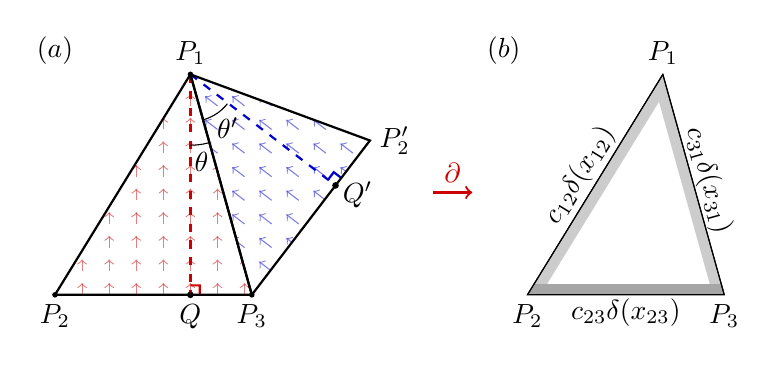
\begin{tikzpicture}
  % 在 (0,0) 处插入图片,宽度设为3cm
  %\node at (0,0) {\includegraphics[width=6.5cm]{FigSchematicFEM02.png}};
  %\node at (4,0) {\includegraphics[width=4cm]{FigSchematicFEM02.png}};


 \coordinate (PS) at (0, 0);
 \coordinate (P2) at ($(0, 0) + (PS)$);
 \coordinate (P3) at ($(\Width, 0) + (PS)$);
 \coordinate (P1) at ($(\Width * 0 .688, \Height) + (PS)$);
 \coordinate (PP) at ($(1.6*\Width, 0.7*\Height) + (PS)$);

\coordinate (C) at (P3);
\coordinate (A) at (P1);
\coordinate (B) at (P2);


\coordinate (F) at ($(C)!(A)!(B)$);
 

  % 画垂线
  \draw[myred,thick, dashed] (A) -- (F);

  \path (P2); \pgfgetlastxy{\ax}{\ay}
  \path (P3); \pgfgetlastxy{\bx}{\by}

   \fill (F) circle(1.2pt) node[below] {$Q$};

  % 计算距离和角度
  \pgfmathsetmacro{\distance}{veclen(\bx-\ax, \by-\ay)}
  \pgfmathsetmacro{\angle}{atan2(\by-\ay, \bx-\ax)}

\path (F); \pgfgetlastxy{\Fx}{\Fy}

\pgfmathsetmacro{\fx}{\Fx/28.453}
\pgfmathsetmacro{\fy}{\Fy/28.453}

\pgfmathsetmacro{\x}{\fx + \De*cos(\angle)}
\pgfmathsetmacro{\y}{\fy + \De*sin(\angle)}
\coordinate (F1) at (\x, \y);

\pgfmathsetmacro{\x}{\fx + 1.41421356*\De*cos(\angle + 45)}
\pgfmathsetmacro{\y}{\fy + 1.41421356*\De*sin(\angle + 45)}
\coordinate (F2) at (\x, \y);

\pgfmathsetmacro{\x}{\fx + \De*cos(\angle + 90)}
\pgfmathsetmacro{\y}{\fy + \De*sin(\angle + 90)}
\coordinate (F3) at (\x, \y);


\draw[myred, thick] (F1) -- (F2) -- (F3);

\begin{scope}
    \clip (P2) -- (P3) -- (P1) -- cycle;
    % 箭头密度参数
    \def\dx{0.344}
    \def\dy{0.3}
    \def\arrowL{0.15}
    % 扫描覆盖整个三角形的矩形网格
    \foreach \x in {0,\dx,...,4}
      \foreach \y in {0,\dy,...,3} {
        \draw[->, >=to, myred, opacity=0.5] (\x,\y) -- ++(0,\arrowL);
      }
\end{scope}

\coordinate (O) at ($(P1) + (0, -0.9)$);
\draw (O) arc [start angle = 270, end angle = 285, radius = 0.9];
\node[xshift = 4, yshift = -6] at (O) {$\theta$};


%%%%%%%%%%%%%%%%%%%%%%%%%%%%%%%%%%%%%%%%%%%%%%%%%%%%%%%%%%%%%%%%%%%%%%%%%%%%%%%%%%%%%%%%%%%%%%%%%%%%%%%%%%%%
\coordinate (C) at (P3);
\coordinate (A) at (P1);
\coordinate (B) at (PP);


\coordinate (F) at ($(C)!(A)!(B)$);
 

  % 画垂线
  \draw[myblue,thick, dashed] (A) -- (F);

  \path (P3); \pgfgetlastxy{\ax}{\ay}
  \path (PP); \pgfgetlastxy{\bx}{\by}

  % 计算距离和角度
  \pgfmathsetmacro{\distance}{veclen(\bx-\ax, \by-\ay)}
  \pgfmathsetmacro{\angle}{atan2(\by-\ay, \bx-\ax)}

 \fill (F) circle(1.2pt) node[below, xshift = 8, yshift = 5] {$Q^\prime$};

\path (F); \pgfgetlastxy{\Fx}{\Fy}

\pgfmathsetmacro{\fx}{\Fx/28.453}
\pgfmathsetmacro{\fy}{\Fy/28.453}

\pgfmathsetmacro{\x}{\fx + \De*cos(\angle)}
\pgfmathsetmacro{\y}{\fy + \De*sin(\angle)}
\coordinate (F1) at (\x, \y);

\pgfmathsetmacro{\x}{\fx + 1.41421356*\De*cos(\angle + 45)}
\pgfmathsetmacro{\y}{\fy + 1.41421356*\De*sin(\angle + 45)}
\coordinate (F2) at (\x, \y);

\pgfmathsetmacro{\x}{\fx + \De*cos(\angle + 90)}
\pgfmathsetmacro{\y}{\fy + \De*sin(\angle + 90)}
\coordinate (F3) at (\x, \y);


\draw[myblue, thick] (F1) -- (F2) -- (F3);


\begin{scope}
    \clip (P1) -- (P3) -- (PP) -- cycle;
    % 箭头密度参数
    \def\dx{0.344}
    \def\dy{0.3}
    \def\arrowL{0.2}
    \pgfmathsetmacro{\Dx}{\arrowL*cos(\angle + 90)}
    \pgfmathsetmacro{\Dy}{\arrowL*sin(\angle + 90)}
    % 扫描覆盖整个三角形的矩形网格
    \foreach \x in {0,\dx,...,4}
      \foreach \y in {0,\dy,...,3} {
        \draw[->, >=to, myblue, opacity=0.5] (\x,\y) -- ++(\Dx, \Dy);
      }
\end{scope}

 \path (P1); \pgfgetlastxy{\ax}{\ay}
  \path (P3); \pgfgetlastxy{\bx}{\by}

  % 计算距离和角度
  \pgfmathsetmacro{\distance}{veclen(\bx-\ax, \by-\ay)}
  \pgfmathsetmacro{\angle}{atan2(\by-\ay, \bx-\ax)}

  \pgfmathsetmacro{\Dx}{0.6*cos(\angle)}
  \pgfmathsetmacro{\Dy}{0.6*sin(\angle)}

\coordinate (O) at ($(P1) + (\Dx, \Dy)$);
\draw (O) arc [start angle = \angle, end angle =\angle + 36, radius = 0.6];
\node[xshift = 9, yshift = -3] at (O) {$\theta^\prime$};



 \node[above] at (P1) {$P_1$};
 \node[below] at (P2) {$P_2$};
 \node[below] at (P3) {$P_3$};
 \node[right] at (PP) {$P_2^\prime$};

\fill (P1) circle (1pt);
\fill (P2) circle (1pt);
\fill (P3) circle (1pt);


  % 可加边框
  \draw[thick] (P1) -- (P2) -- (P3) -- cycle;
  \draw[thick] (P3) -- (PP) -- (P1) -- cycle;

 

%%%%%%%%%%%%%%%%%%%%%%%%%%%%%%%%%%%%%%%%%%%%%%%%%%%%%%%%%%%%%%%%%%%%%%%%%%%%%%%%%%%%%%%%%%%%%%%%%%%%%%%%%%%%%%%%%%%%%%%%%%%%%%%%%%%%

\coordinate (PS) at (6, 0);
 \coordinate (P2) at ($(0, 0) + (PS)$);
 \coordinate (P3) at ($(\Width, 0) + (PS)$);
 \coordinate (P1) at ($(\Width * 0 .688, \Height) + (PS)$);


 \begin{scope}
    \clip (P2) -- (P3) -- (P1) -- cycle;
    % 箭头密度参数
   \draw[gray!40, line width=8.0] (P1) -- (P2);
\draw[gray!40, line width=8.0] (P1) -- (P3);
\draw[gray!70, line width=8.0] (P2) -- (P3);
  \end{scope}

  \draw (P1) -- (P2) node[midway, above, sloped, yshift = -2] {$c_{12}\delta(x_{12})$};
\draw (P1) -- (P3) node[midway, above, sloped, yshift = -3] {$c_{31}\delta(x_{31})$};
\draw (P2) -- (P3) node[midway, below, sloped, yshift = 2] {$c_{23}\delta(x_{23})$};
 
   \draw[] (P1) -- (P2) -- (P3) -- cycle;

   \node[above] at (P1) {$P_1$};
 \node[below] at (P2) {$P_2$};
 \node[below] at (P3) {$P_3$};

%%%%%%%%%%%%%%%%%%%%%%%%%%%%%%%%%%%%%%%%%%%%%%%%%%%%%%%%%%%%%%%%%%%%%%%%%%%%%%%%%%%%%%%%%%%%%%%%%%%%%%%%%%%%%%%%%%%%%%%%%%%%%%%%%%%
 \node at (0, \Height + 0.3) {$(a)$};
\node at (5.7, \Height + 0.3) {$(b)$};

\draw[->, >=to, thick, color = myred] (4.8, 1.3) -- (5.3,1.3) 
    node[midway, above, sloped] {$\partial$};
   
\end{tikzpicture}
\end{document}